\documentclass[../main.tex]{subfiles}

\begin{document}
\section{UCB-BAR: Rocket Chip Generator}
\label{sec:RCG}
\begin{figure}
    \centering
    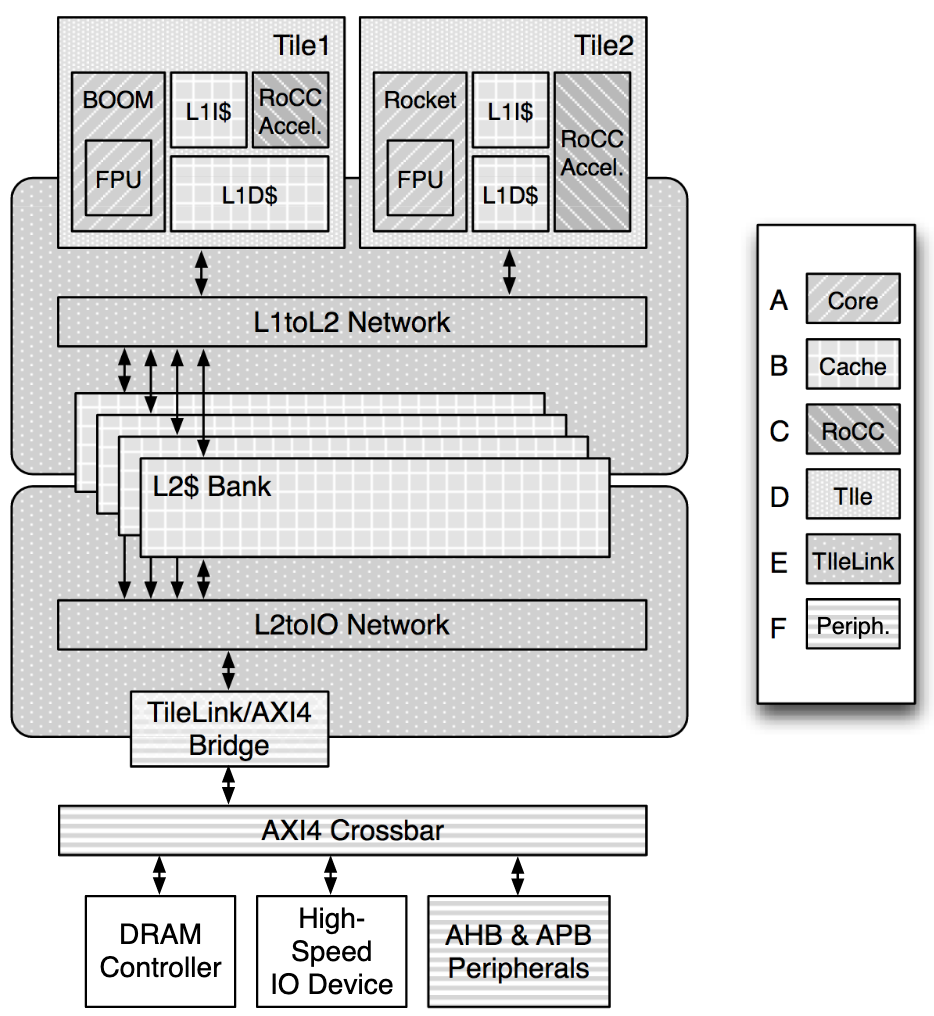
\includegraphics[scale=.35]{pngs/RocketChipGeneratorLayout.png}
    \caption{Generic Rocket Chip\cite{Asanović:EECS-2016-17}}
    \label{fig:RocketCipGen}
\end{figure}

In any standalone system, there must be a host controller, and in CHIPS architecture, the ASICs are not capable of being standalone. The host controller would need high-level programming support and be relatively mature. The UCB-BAR's RCG is a perfect fit for this architecture. It fully supports the reduce instruction set computer version five (RISC-V) Instruction Set Architecture (ISA). The RCG has been taped out eleven times and in various process nodes. The Chip Alliance foundation maintains the RCG. It creates an SoC with caches and tiles, and figure \ref{fig:RocketCipGen} shows the layout of a generic Rocket chiplet. 

\subsection{Generic Rocket Chip}
The lowest layer in the system is the tile layer. This layer is where the processor,  L1 instruction, and L1 data cache reside. In addition to these modules, a tile can instantiate a rocket custom co-processor (RoCC).  The tile defaults to one of the following cores: Rocket core, or Berkeley out of order machine (BOOM) core.  The next layer is the L2 caches layer, which connects through the L1toL2 tile link memory bus to the tiles. The top layer is the IO layer, which connects through L2toIO tile link memory bus to the L2 caches. The Rocket chiplet's IO consists of one advanced extensible interface (AXI) bus and one host bus. The host bus uses the direct memory interface (DMI) protocol to interface with the off-chip host system. 


\subsection{Rocket Core}
\begin{figure}
    \centering
    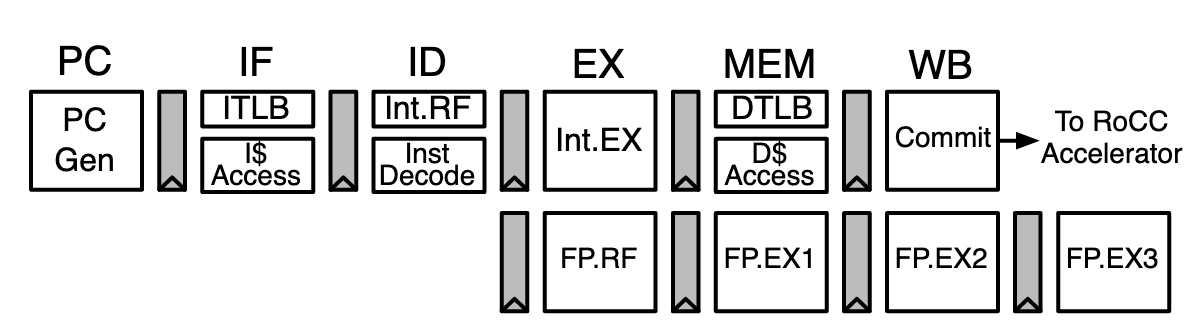
\includegraphics[scale=.35]{pngs/RocketPipeline.png}
    \caption{Rocket Chip Pipeline\cite{Asanović:EECS-2016-17}}
    \label{fig:RocketCipFlow}
\end{figure}
This RISC-V based Rocket core is a single fetch, single issue, in-order scalar processor. Fig. \ref{fig:RocketCipFlow} shows the pipeline for this processor. It supports the IMAFD extensions of the RISC-V (ISA)\cite{RISC-V-isa}. IMAFD extensions represent the following functionality: integer (I), multiply and divide (M), atomic (A), single-precision (F), and double-precision (D) floating-point\cite{RISC-V-isa}. In addition to the IMAFG extension, it supports the E extension\cite{RISC-V-isa}. This extension stands for the custom extension and is used to communicate with the RoCC unit.

\subsection{Chisel}
The RCG uses the hardware construction language (HCL) Chisel\cite{chisel:book}. It embeds itself into the Scala programming language. Because of the Scala language, it gains a high-level of abstraction, and sophisticated hardware designs become more simplistic to design\cite{chisel:book}. This achieves its goal to merge hardware development with software development and enables complex function to drive how hardware is created, which is not currently possible in low-level hardware description languages (HDL)\cite{chisel:book}.

\end{document}